%  % XeLaTeX document
% \documentclass[12pt,a4paper]{article}

% % Редактируем: конфигурация, личные настройки: имя, название предмета и пр. для титульной страницы и метаданных документа здесь
% \newcommand{\university}{Санкт-Петербургский политехнический университет Петра Великого}
\newcommand{\faculty}{Институт физики, нанотехнологий и телекоммуникаций}
\newcommand{\department}{Высшая инженерно-физическая школа}
\newcommand{\city}{Санкт-Петербург}
\newcommand{\num}{}
\newcommand{\docname}{Отчет по лабораторной работе №1}
\newcommand{\subject}{Молекулярное моделирование}
\newcommand{\tutorname}{И. М. Соколов}
\newcommand{\studentname}{В. Х. Салманов}
\newcommand{\group}{3430302/60201}

% % Не редактируем: используемые пакеты
% % настройка кодировки, шрифтов и русского языка
\usepackage{fontspec}
\usepackage{polyglossia}

% рабочие ссылки в документе
\usepackage{hyperref}

% графика
\usepackage{graphicx}
\usepackage{tikz}

% поворот страницы
\usepackage{pdflscape}

% качественные листинги кода
\usepackage{minted}
\usepackage{listings}
\usepackage{lstfiracode}

% отключение копирования номеров строк из листинга, работает не во всех просмотрщиках (в Adobe Reader работает)
\usepackage{accsupp}
\newcommand\emptyaccsupp[1]{\BeginAccSupp{ActualText={}}#1\EndAccSupp{}}
\let\theHFancyVerbLine\theFancyVerbLine
\def\theFancyVerbLine{\rmfamily\tiny\emptyaccsupp{\arabic{FancyVerbLine}}}

% библиография
\bibliographystyle{templates/gost-numeric.bbx}
\usepackage{csquotes}
\usepackage[parentracker=true,backend=biber,hyperref=false,bibencoding=utf8,style=numeric-comp,language=english,autolang=other,citestyle=gost-numeric,defernumbers=true,bibstyle=gost-numeric,sorting=ntvy,]{biblatex}

% установка полей
\usepackage{geometry}

% нумерация картинок по секциям
\usepackage{chngcntr} 

% дополнительные команды для таблиц
\usepackage{booktabs}

% для заголовков
\usepackage{caption} 
\usepackage{titlesec}
\usepackage[dotinlabels]{titletoc}

% разное для математики
\usepackage{amsmath, amsfonts, amssymb, amsthm, mathtools}
\usepackage{braket}


% водяной знак на документе, см. main.tex
\usepackage[printwatermark]{xwatermark} 

% использование различных спец. символов
\usepackage{gensymb}

% таблицы
\usepackage{tabularx}
\newcolumntype{Y}{>{\centering\arraybackslash}X}

% гиперссылки
\usepackage{hyperref}

% межстрочный интервал
\sloppy
\linespread{1.2}
\usepackage{multirow}
\usepackage{graphicx}

\usepackage{import}

% % Не редактируем: параметры используемых пакетов и не только
% % настройки polyglossia
\setdefaultlanguage{russian}
\setotherlanguage{english}

% локализация
\addto\captionsrussian{
  \renewcommand{\figurename}{Рисунок}%
  \renewcommand{\partname}{Глава}
  \renewcommand{\contentsname}{\centerline{Содержание}}
  \renewcommand{\listingscaption}{Листинг}
}

% основной шрифт документа
\setmainfont{CMU Serif}

% перечень использованных источников
\addbibresource{refs.bib}

% настройка полей
\geometry{top=2cm}
\geometry{bottom=2cm}
\geometry{left=3cm}
\geometry{right=1.5cm}
\geometry{bindingoffset=0cm}

% настройка ссылок и метаданных документа
\hypersetup{unicode=true,colorlinks=true,linkcolor=red,citecolor=green,filecolor=magenta,urlcolor=cyan,
    pdftitle={\docname},   	    
    pdfauthor={\studentname},      
    pdfsubject={\subject},      		        
    pdfcreator={\studentname}, 	       
    pdfproducer={Overleaf}, 		     
    pdfkeywords={\subject}
}

% настройка подсветки кода и окружения для листингов
\usemintedstyle{colorful}
\newenvironment{code}{\captionsetup{type=listing}}{}

% шрифт для листингов с лигатурами
\setmonofont{FiraCode-Regular.otf}[
    Path = templates/,
    Contextuals=Alternate
]

% оформления подписи рисунка
\captionsetup[figure]{labelsep = period}

% подпись таблицы
\DeclareCaptionFormat{hfillstart}{\hfill#1#2#3\par}
\captionsetup[table]{format=hfillstart,labelsep=newline,justification=centering,skip=-10pt,textfont=bf}

% путь к каталогу с рисунками
\graphicspath{{fig/}}

% Внесение titlepage в учёт счётчика страниц
\makeatletter
\renewenvironment{titlepage} {
 \thispagestyle{empty}
}
\makeatother

\counterwithin{figure}{subsection}
\counterwithin{table}{subsection}

\titlelabel{\thetitle.\quad}

% для удобного конспектирования математики
\mathtoolsset{showonlyrefs=true}
\theoremstyle{plain}
\newtheorem{theorem}{Теорема}[subsection]
\newtheorem{proposition}[theorem]{Утверждение}
\theoremstyle{definition}
\newtheorem{corollary}{Следствие}[theorem]
\newtheorem{problem}{Задача}[subsection]
\theoremstyle{remark}
\newtheorem*{nonum}{Решение}

% настоящее матожидание
\newcommand{\MExpect}{\mathsf{M}}

% объявили оператор!
\DeclareMathOperator{\sgn}{\mathop{sgn}}

% перенос знаков в формулах (по Львовскому)
\newcommand*{\hm}[1]{#1\nobreak\discretionary{} {\hbox{$\mathsurround=0pt #1$}}{}} 

% формулы
\newcommand{\mequation}[1]{
\begin{equation}
\begin{split}
\begin{gathered}
#1
\end{gathered}
\end{split}
\end{equation}
}

% % водяной знак для обозначения статуса документа
% %\newwatermark[allpages,color=red!40,angle=45,scale=3,xpos=0,ypos=0]{DRAFT}

% \begin{document}
% % Не редактируем: Титульная страница (формируется автоматически из заданной конфигурации)
% \begin{titlepage}	% начало титульной страницы

	\begin{center}		% выравнивание по центру

		\large \university \\
		\large \faculty \\
		\large \department \\[5cm]
		% название института, затем отступ 6см
		
		\LARGE \textbf \subjecttype \\ % тип работы (например: курсовая работа)
		\LARGE \subject \\[0.5cm] % название работы, затем отступ 0,5см
		\large \docname \num \\[4.1cm]
		%\large Тема работы\\[5cm]

	\end{center}


	\begin{flushright} % выравнивание по правому краю
		\begin{minipage}{0.25\textwidth} % врезка в половину ширины текста
			\begin{flushleft} % выровнять её содержимое по левому краю

				\large\textbf{Работу выполнил:}\\
				\large \studentname \\
				\large {Группа:} \group \\
				
				\large \textbf{Преподаватель:}\\
				\large \tutorname

			\end{flushleft}
		\end{minipage}
	\end{flushright}
	
	\vfill % заполнить всё доступное ниже пространство

	\begin{center}
	\large \city \\
	\large \the\year % вывести дату
	\end{center} % закончить выравнивание по центру

\end{titlepage} % конец титульной страницы

\vfill % заполнить всё доступное ниже пространство


% % Не редактируем: Страница содержания (формируется автоматически из section, subsection и пр., указанных в content.tex)
% % Содержание
\setcounter{tocdepth}{1} % Show sections
\setcounter{tocdepth}{2} % + subsubsections
\setcounter{tocdepth}{3} % + paragraphs
\setcounter{tocdepth}{4} % + paragraphs
\setcounter{tocdepth}{5} % + subparagraphs
\tableofcontents
\newpage



% % Редактируем: всё остальное: вступление, др. этапы, заключение, приложение
\section{Цель работы}
Найти седловую точку первого порядка молекулы трифторметанола.

\section{Постановка задач}
Найти ES молекулы трифторметанол методом B3LYP/6-31G. Предположить вид TS данной молекулы. Провести оптимизацию TS методом B3LYP/6-31G и привести следующие результаты:
\begin{itemize}
    \item[-] энергия ES, Ts и вклады в них;
    \item[-] высота потенциального барьера
    \item[-] определить, может ли этот барьер преодолеваться термически при комнатной температуре
\end{itemize}

\begin{figure}[H]
\centering
\captionsetup{justification=centering}
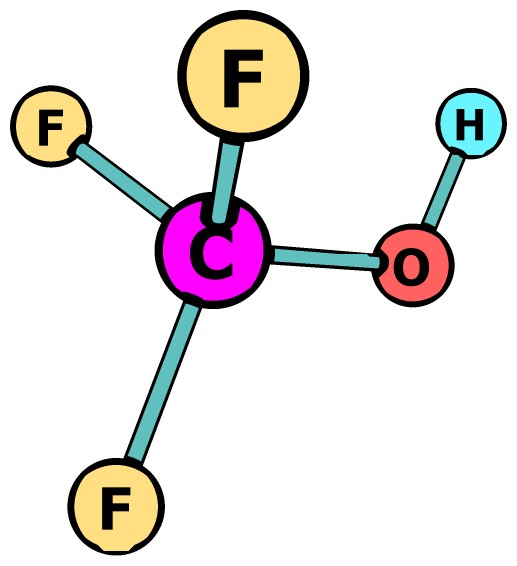
\includegraphics[scale=0.4]{fig/0.jpg}
\caption{Молекулы трифторметанол}
\end{figure}
\section{Теоретическая информация}
\subsection{Поверхность потенциальной энергии}
Теоретической моделью для описания химических процессов является поверхность потенциальной энергии (ППЭ). Понятие ППЭ вводится в рамках приближения Борна-Оппенгеймера, в котором предполагается, что в связи с сохранением импульса молекулярной системы и существенным превышением массы ядра над массой электрона, атомные ядра покоятся в сравнении с "быстрыми" электронами. Таким образом, электроны мгновенно подстраиваются под любое изменение ядер, и можно разделять движение электронов и ядер. В данном приближении под ППЭ понимают энергию молекулярной системы, равную \textit{сумме энергии электронов (одно- и двуэлектронные интегралы) при данной конфигурации ядер и энергии кулоновского отталкивания ядер}, записанную как функцию координат ядер $E(\vec{R})$. 

Для анализа характеристик ППЭ используют матрицу первых производных энергии по координатам ядер (градиент энергии):
\mequation{
    \left(
        \frac{\partial E}{\partial q_1}, \frac{\partial E}{\partial q_2}, \ldots, \frac{\partial E}{\partial q_{3N - 6}}  
    \right)
}
где $N$ - число атомов в системе, $\{q_i\}_{i=1}^{3N-6}$ - нормальные координаты.

Те точки, в которых все компоненты градиента равны нулю, называют критическими точками. Это могут могут быть минимумы, максимумы или седловые точки. 

Для определения типа критической точки необходимо знать матрицу вторых производных энергии по координатам ядер (матрица Гессе, гессиан):
\mequation{
    H_{ij} = \left( \frac{\partial^2 E}{\partial q_i \partial q_j} \right)
}

Если все собственные числа \textbf{H} положительны, то критическая точка является минимумом (глобальным или локальным). В случае если одно из собственных чисел \textbf{H} отрицательно, то критическая точка является седловой точкой первого порядка.

\subsection{Методы поиска седловых точек}
В настоящее время существует ряд методов поиска седловых точек:
\begin{enumerate}
    \item требующие начального приближения для переходного состояния;
    \item требующие угадывания реакционных координат (relaxed scan);
    \item требующие угадывания реагентов и продуктов реакции (nudged elastic band method, string method, growing string method);
    \item не требующие угадывания и следующие реакциям вида $A \leftrightarrow X(+Y)$ для локального минимума A (ADDF);
    \item не требующие угадывания и следующие реакциям вида $A + B \leftrightarrow X(+Y)$ для нескольких реагентов A и B (AFIR).
\end{enumerate}

В данной работе будет использован первый подход.

\begin{figure}[H]
\centering
\captionsetup{justification=centering}
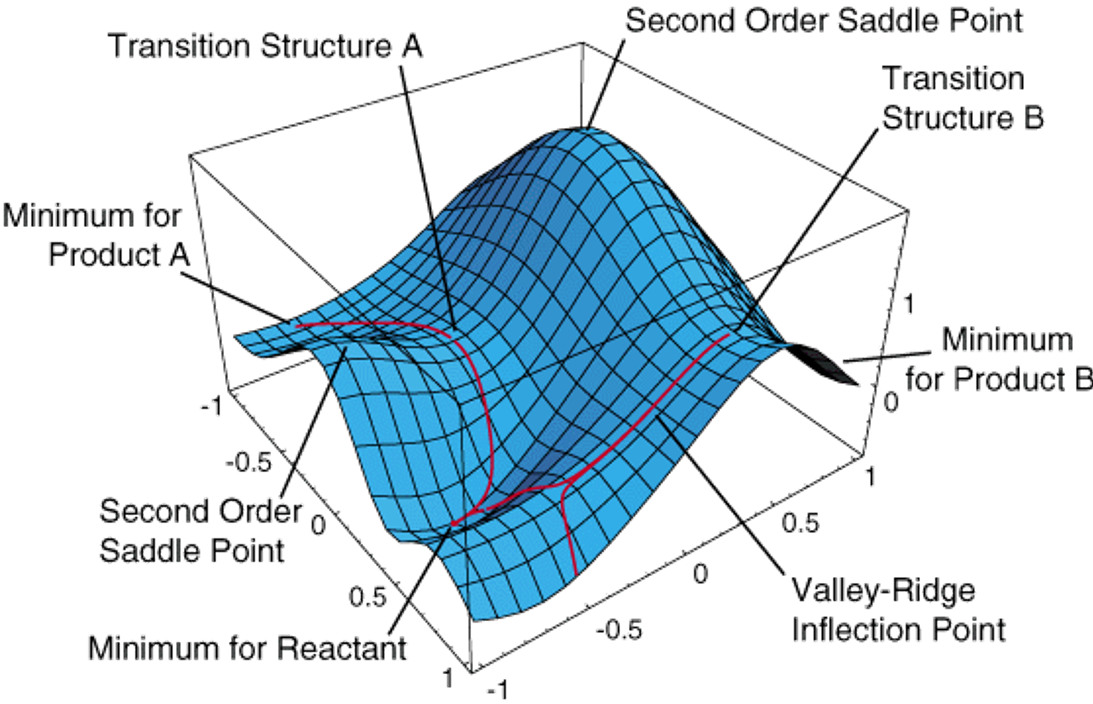
\includegraphics[scale=0.8]{fig/2.png}
\caption{ППЭ и важный точки на ней.}
\end{figure}
    
\section{Результаты}
Для нейтральной и депротонированной форм молекулы была проведена оптимизация методом B3LYP/6-31G. В полученных минимумах были проведены SP-вычисления методом B3LYP/6-311G++(2d,p).

\begin{table}[H]
    \caption{Значения энергии для форм молекулы (в Хартри)} 
    \label{tab:my-table}
        \begin{center}
            \begin{tabular}{|c|c|c|}
            \hline
            Форма соединения & \begin{tabular}[c]{@{}c@{}}Полная энергия\\ с учетом сольватации\end{tabular} & Энергия сольватации \\ \hline
            Нейтральная & -433.538121 & -0.019305 \\ \hline
            Депротонированная & -433.090787 & -0.096514 \\ \hline
            \end{tabular}
        \end{center}
\end{table}

Вычислим значение $pK_a$.
\mequation{
    D = E^{-} - E^{0} = 0.447334 \\
    \left(pK_a\right)_{T} = 1.23
}

Экспериментальное значение $pK_a = 1.68$\footnote{\url{https://pubchem.ncbi.nlm.nih.gov/bioassay/448096#sid=103702226&section=Version}}
\section{Выводы}
В данном соединении преобладают $n-\pi$-переходы. Соединение поглощает в диапазоне длин волн от 200 до 400 нм. Максимум поглощения приходится на 247 нм.
\section{Контроль результатов}
\begin{itemize}
    \item в выходных файлах содержатся “EQUILIBRIUM GEOMETRY LOCATED” и “SADDLE POINT LOCATED”;
    \item энергия TS выше энергии ES.
\end{itemize}{}
\section{Приложенные файлы}
\begin{itemize}
    \item struct.mol – исходная структура;
    \item TDDFT.inp – входной файл;
    \item TDDFT.log – выходной файл.
\end{itemize}{}

% % Не редактируем: Страница библиографии (формируется автоматически из книжек, указанных в refs.bib и пометок \cite{имя_источника} в тексте)
% \newpage
\printbibliography[title=Перечень использованных источников]
\addcontentsline{toc}{subsection}{Перечень использованных источников}
% \end{document}
